\section{ESPml Schema}

\subsection{Purpose and Goals}

The purpose of the ESPml schema language is to define a standard
protocol with which the different entities in the framework 
can communicate and also to have a unifying grammar that systems 
can describe their abilities. ESPml is held very generic such that it
can describe a lot of different systems like databases, sensor
networks, weather stations or even web cameras.

\subsection{Components}

The different components in ESPml describe the different parts of a
system. The main entity is the system element. The system element
contains one or more fields, which are a collection of one or more
platforms. And finally, a platform is a collection of sensors, the
smallest entity possible. We will now go into details of each of the
elements.

\subsubsection{System}
\begin{figure}[t]
  \begin{center}
    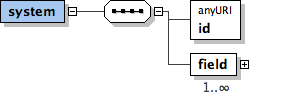
\includegraphics[width=0.33\textwidth]{images/system}
    \caption{Model view of the system component in the ESPml schema.}
    \label{fig:system}
  \end{center}
\end{figure}
Figure \ref{fig:system} depicts the model view of the top-level
element of the schema, the system component. The system consists of an
id element of type anyURI and one or more field elements. The id
element points to the address where the system's web services can be
reached, i.e., where one can execute remote functions through web
service calls. The field elements represent actual sensor
networks. For example, if a system has multiple physical deployments,
and there is one common interface for all the fields in the system,
then the different deployments can be represented as different
fields. We will describe the field element in the next section.


\subsubsection{Field}
\begin{figure}[t]
  \begin{center}
    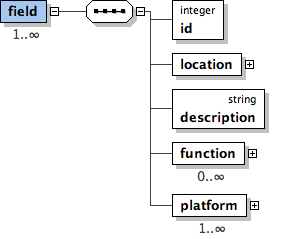
\includegraphics[width=0.39\textwidth]{images/field}
    \caption{Model view of the field component in the ESPml schema.}
    \label{fig:field}
  \end{center}
\end{figure}
Illustrated in Figure \ref{fig:field} is the field element of
ESPml. The field consists of an id of type integer. This id should be
unique within the system and is used to identify the field. The
location can be a point or a polygon which describes the physical
location of the field. We will describe the location element in more
detail in Section \ref{sec:location}. Each field has a description
element of type string which describes the type and purpose of the
field in a verbal manner. A field can also have zero or more functions
associated with it. In general, these functions should act on
the whole field, for example, they could return the average value of a
sensor reading over the whole field, etc. The last element in a field
is one or more platforms.


\subsubsection{Platform}
\begin{figure}[t]
  \begin{center}
    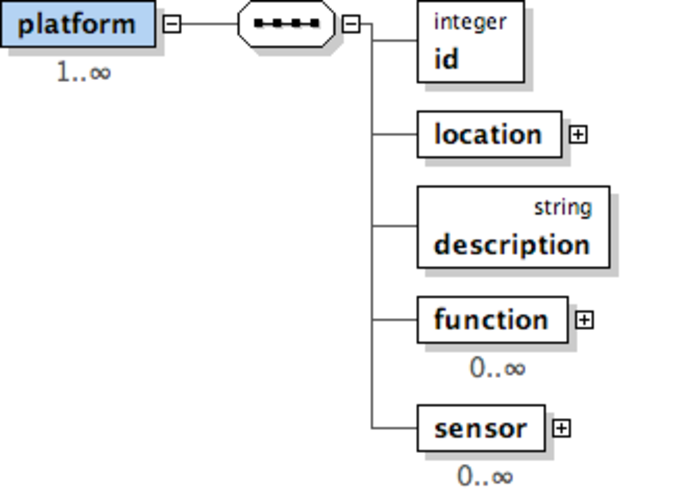
\includegraphics[width=0.39\textwidth]{images/platform}
    \caption{Model view of the platform component in the ESPml schema.}
    \label{fig:platform}
  \end{center}
\end{figure}
Figure \ref{fig:platform} shows the model view of the platform
element. A platform element represents a physical entity with a
micro-controller, some communication device and a possible energy
source. The integer id in a platform has to be unique within the
field. Thus, the field id and the platform id can uniquely identify
any platform in the system. Each platform has a location, a
string description, and functions which can be executed.  These functions can 
affect the
platform for actuation purposes, retrieve data values such as the exact
location, the local time at the platform, or to move the platform
around. Each platform also contains zero or more sensors.


\subsubsection{Sensor}
\begin{figure}[t]
  \begin{center}
    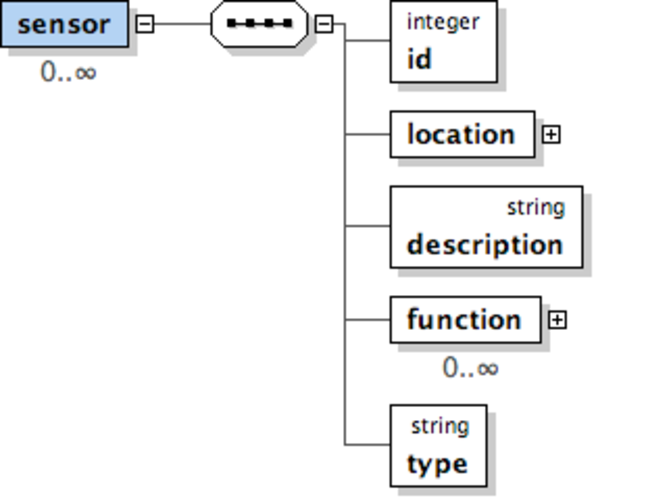
\includegraphics[width=0.39\textwidth]{images/sensor}
    \caption{Model view of the sensor component in the ESPml schema.}
    \label{fig:sensor}
  \end{center}
\end{figure}
Probably the most important component of the ESPml schemas is the sensor. 
Figure \ref{fig:sensor} depicts the model view. The sensor
element represents a sensor on a platform, such as a thermistor,
light-sensor, camera, etc. The id must be unique on the
platform. Similar to the other elements, the sensor element has a
location, description, and function element. One additional important
element is the type element which describes the type of sensor. This
type is not standardized right now, and can thus be defined by the system
developer.  This will change in the future since we intend to provide a standard for describing
sensor types.

\subsection{Descriptions}
The next four sections will explain the different additional fields
for the field, platform and sensor element in more detail. 

\subsubsection{Location}\label{sec:location}
The location element describes, as the name suggests, the location of
the enclosing element. The location is described either by a point or
a polygon element. The point element contains a simple string of the
format ``$latitude$, $longitude$, $altitude$'' and is derived from the
GML standard. The polygon is composed of a multi line string, where
each line represents a corner of the polygon and is also derived from
the GML standard. The format for each line is the same as the point
element. Additionally, the polygon has to be closed, i.e., the first
and last point have to coincide.

\subsubsection{Functions}\label{sec:function}
\begin{figure}[t]
  \begin{center}
    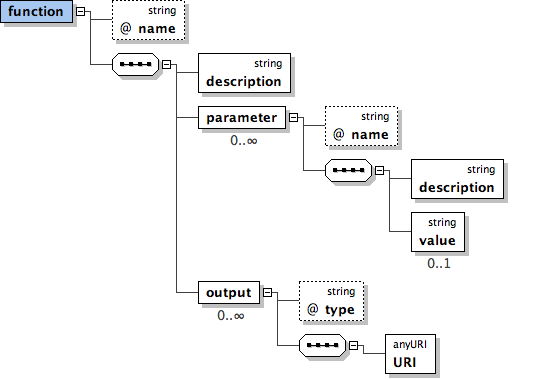
\includegraphics[width=0.49\textwidth]{images/function}
    \caption{Model view of the function element in the ESPml schema.}
    \label{fig:function}
  \end{center}
\end{figure}
The function element is a little bit more complicated than the other
elements.  The location of the function within the XML determines to
which component it is attributed to. For example, a function in the field
element should affect the whole field, whereas a function in a
platform element should affect only that platform.

Figure \ref{fig:function} depicts its model view. Each function has a
name attribute. The name attribute should be reflective of the
function's purpose. For example, a function which returns a sensor's
data, should be called \verb|getSensorData|, a function which sets the
sampling rate of a sensor, should be called \verb|setSamplingRate|,
etc. We do not enforce a naming schema for functions. Though we
encourage the user to choose meaningful names. In a later version we
will develop a standard naming schema for commonly used functions.

Each function element contains a description which
details what the function actually does. Additionally,
a function element contains zero or more parameter elements and zero or more
output elements. What role they play will be explained in the
following example where we show how one defines, executes and then collects the
data from a function.

\begin{itemize}
\item \textbf{Declaring a Function}

The function declaration is done in the system's XML schema file which
is sent to the registry. Each field, platform, and sensor should
define the functions it supports, including each function name
attribute, the description element, and the parameter elements with
name and description, which need to be provided to execute the
function later on. The following code example is an excerpt of a ESPml
XML file a system sends to the registry, and defines a sensor with
two functions. The first function gets the current sensor value and has no
parameter. The second function gets the average value over a certain number
of recorded data. Thus, it needs a parameter which tells the function
how many elements it should calculate the average.

\lstset{basicstyle=\small,breaklines=true}
\begin{lstlisting}
...
<sensor>
  <id>1</id>
  <location>
    <point>
      <pos>34.0682,-118.44,0.00</pos>
    </point>
  </location>
  <description>PhotoSensor</description>
  <function name="getCurrentValue">
    <description>Get the current value for this sensor.
    </description>
  </function>
  <function name="getAverageValue">
    <description>Gets the average for this sensor.
    </description>
    <parameter name="numberElements">
      <description>The number of elements for which the average should be calculated.
      </description>
    </parameter>
  </function>
  <type>Light</type>
</sensor>
...
\end{lstlisting}


\item \textbf{Executing a Function}

If a client wants to execute a function, then it sends a ESPml XML
file to the system's URI. In the XML file, the user will add the function
element that needs to be executed on a field, platform, or sensor. 
It is also possible to execute multiple functions in one
request. The following listing shows parts of a ESPml XML file which
a client sends to a system to execute functions. This excerpt will
execute \verb|getAverageValue| on platform 1, sensor 1 with a
parameter value of 10, and it will get the current value of platform
2's sensor 1.

\lstset{basicstyle=\small,breaklines=true}
\begin{lstlisting}
...
<platform>
  <id>1</id>
  <sensor>
    <id>1</id> 
    <function name="getAverageValue">
      <parameter name="numberElements">
        <value>10</value>
      </parameter>
    </function>
  </sensor>
<platform>
<platform>
  <id>2</id>
  <sensor>
    <id>1</id> 
    <function name="getCurrentValue">
    </function>
  </sensor>
<platform>
...
\end{lstlisting}

\item \textbf{Collecting Function Output}

The system will respond with another ESPml XML file which will be
filled with the output elements of the received function calls. The output
elements consist of a type attribute and a URI field. The type element
describes the mime-type of the file the URI points to. The following
listing is an example response to the function executed from the last
example. 


\lstset{basicstyle=\small,breaklines=true}
\begin{lstlisting}
...
<platform>
  <id>1</id>
  <sensor>
    <id>1</id> 
    <function name="getAverageValue">
      <output type="text/comma-separated-values">
        <URI>http://foobar.org:8080/sensor_getAverageValue/852760e7177ac9eeebcc16621ec2e83c
	</URI>
      </output>
    </function>
  </sensor>
<platform>
<platform>
  <id>2</id>
  <sensor>
    <id>1</id> 
    <function name="getCurrentValue">
      <output type="text/comma-seperated-values">
        <URI>http://foobar.org:8080/sensor_getCurrentValue/76344f22bdbc47211407b085bf5da147
	</URI>
      </output>
    </function>
  </sensor>
<platform>
...
\end{lstlisting}

\end{itemize}


\subsubsection{Mobility}
The location element has an optional element ``mobile''. This
indicates that the enclosing element is mobile and can move
around. This is an indicator that the location might not be the real
location where the element is right now and that one has to take some
precaution. In the future, we will require a special function to get
the enclosing elements exact current location if the mobile element is
defined.


\subsubsection{Additional Ideas}
The current ESPml schema is not complete and is open for further
development. It has all the functionality to get a simple example
system up and running but it will be extended in the future. Some
points which will be addressed are:
\begin{itemize}
\item standards for function names and types
\item confidentiality, privacy, and authentication
\item improved location element for different coordinate systems
\item scalability
\item etc.
\end{itemize}
We have a closer look at these extensions in Section \ref{sec:future_work}.
